%!TEX root = ../dokumentation.tex

\chapter{Konzept}

\section{System-Grundlage und Struktur}
Als Grundlage der Schnittstelle soll eine MATLAB-Standalone-Applikation dienen, welche eine zentrale Benutzeroberfläche für die Funktionalitäten der Anforderungen stellt. Dies ermöglicht das spätere Kompilieren der Applikation und die Möglichkeit diese als einfaches Programm auf einem Rechner zu starten und von hier aus eine Auswahl über die einzelnen Funktionen der Applikation zu bekommen. Zudem kann so die Applikation einfach verteilt und auf mehreren Rechner installiert werden ohne dass zusätzliche Bibliotheken oder Programmierkenntnisse benötigt werden.

Innerhalb der Implementierung ergeben sich zwei große Bereiche in die die Applikation aufgeteilt wird und die beiden Hauptfunktionalitäten der Anforderung, das erstellen geeigneter Samples in Kubios HRV Premium und das grafische Darstellen der erzeugten medizinischen Messdaten, repräsentieren. Diese beiden Hauptfunktionalitäten sollen dazu voneinander abgekapselt implementiert werden, wobei das Visualisieren die Basis der Applikation darstellt und die Konfiguration der Samples auf dieser aufbaut bzw. von hier aus aufgerufen wird.

% vorläufiges Klassendiagramm
\begin{figure}[H]
	\centering
	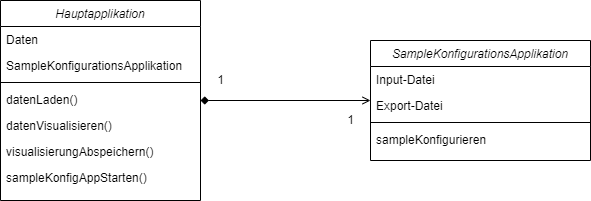
\includegraphics[width=1\linewidth]{konzeptKlassen}
	\caption{Konzept Klassendiagramm}
	\label{fig:konzeptKlassen}
\end{figure}

\section{Ablauf}
Die grundlegenden Benutzung der Applikation soll wie folgt stattfinden. Der Benutzer kann entweder Samples für eine Messung konfigurieren und diese dann im nächsten Schritt innerhalb des Tools visualisieren oder, bei bereits angelegten Samples, diese direkt im Graphen anzeigen. So kann die Erstellung neuer Visualisierungsdaten, aber auch die Wiederverwendbarkeit bereits angelegter Daten gewährleistet werden. Innerhalb eines Ablaufdiagramms lässt sich dies folgendermaßen beschreiben:

\begin{figure}[H]
	\centering
	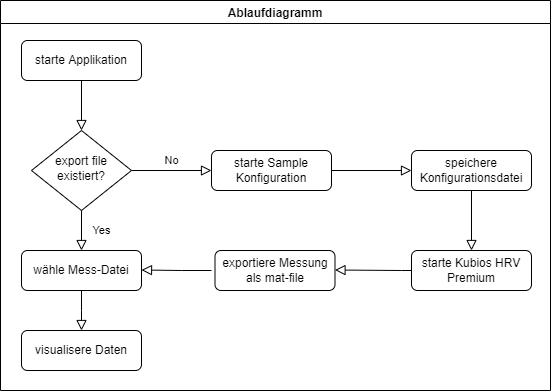
\includegraphics[width=0.8\linewidth]{ablaufKonzept}
	\caption{Ablaufdiagramm des Konzepts}
	\label{fig:ablaufKonzept}
\end{figure}

Für das Erstellen der Samples wurde folgender Ablauf konzipiert. % keine ahnung was hier abgeht

Für das Visualisieren einzelner Messparametern innerhalb der Applikation wird ein Ablauf wie folgt modelliert. Nach dem das in Kubios erstellte MAT-File in die Applikation geladen wird, kann eine der enthaltenen Parameter in einer Liste ausgewählt werden. Die dazugehörigen Messdaten werden dann im bereits vorhandenen Koordinatensystem angezeigt. Das Visualisieren anderer Parameter erfolgt durch das Auswählen eines anderen Listen-Elements. 

\begin{figure}[H]
	\centering
	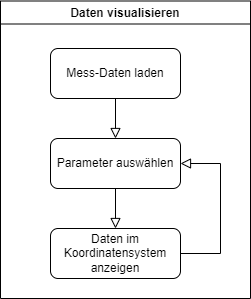
\includegraphics[width=0.35\linewidth]{ablaufVisualisieren}
	\caption{Konzept für das Visualisieren von Daten}
	\label{fig:ablaufVisualisieren}
\end{figure}

\section{Applikations-Design}


% Design-Konzept hinzufügen